
\chapter{Orientación a Objetos}

Pese a la ausencia de objetos según el sistema tradicional de orientación
a objetos, Go es un lenguaje perfectamente orientado a objetos y lo hace de una
forma más lógica según la definición formal de los objetos.

\section{Métodos}

Go no posee clases, pero su ausencia no impide que se puedan crear métodos
específicos para un tipo de datos concreto. Es posible crear métodos para (casi)
cualquier tipo de datos.

	\subsection{Métodos para structs}

	Los métodos en Go se declaran de forma independiente de la declaración del
	tipo. Éstos se declaran como funciones con un receptor explícito. Siguiendo
	con el ejemplo del tipo \textit{Punto}:

	\begin{verbatim} type Punto struct { x, y float }
    
		// Un método sobre *Punto func (p *Punto) Abs() float { return
		math.Sqrt(p.x*p.x + p.y*p.y) } \end{verbatim}

	Cabe notar que el receptor es una variable explícita del tipo deseado (no
	existe puntero a \textit{this}, sino que hay una referencia explícita al
	tipo \textit{*Punto}.\\

	Un método no requiere un puntero a un tipo como receptor, sino que podemos
	usar un tipo pasado como valor. Esto es más costoso, ya que siempre que se
	invoque al método el objeto del tipo será pasado por valor, pero aún así es
	igualmente válido en Go.

	\begin{verbatim} type Punto3 struct { x, y float }
    
		// Un método sobre Punto3 func (p Punto3) Abs() float { return
		math.Sqrt(p.x*p.x + p.y*p.y + p.z*p.z) } \end{verbatim}

	\subsection{Invocación de métodos}

	Los métodos se invocan de una manera muy simple, tal y como se podría
	esperar en cualquier otro lenguaje orientado a objetos.

	\begin{verbatim} p := &Point { 3, 4 } fmt.Print(p.Abs())    // Imprimirá
	5 \end{verbatim}

	Ahora veamos un ejemplo de uso de un ejemplo con un tipo de datos que no sea
	de tipo \textit{struct}.

	\begin{verbatim} type IntVector []int
    
		func (v IntVector) Sum() (s int) { for i, x := range v { s += x } return
		}
    
		fmt.Println(IntVector { 1, 2, 3 }. Sum()) \end{verbatim}

	\subsection{Reglas para el uso de métodos}

	Existen una serie de reglas concernientes a los métodos. Como se ha
	mencionado, los métodos están relacionados con un tipo concreto, digamos
	\textit{Foo}, y están enlazados a su tipo de manera estática.\\

	El tipo de un receptor en un método puede ser tanto \textit{*Foo} como
	\textit{Foo}. Se pueden tener simultáneamente varios métodos \textit{Foo}
	y otros cuantos métodos \textit{*Foo}.\\

	\textit{Foo} Por sí solo no puede ser de tipo puntero, aunque los métodos
	puedan obtener un receptor de tipo \textit{*Foo}.\\

	Por último, hay que tener en cuenta que un tipo \textit{Foo} debe estar
	definido en el mismo paquete que todos sus métodos.

	\subsection{Punteros y valores en los métodos}

	Go automáticamente indirecciona o derreferencia los valores cuando se invoca
	un método. Por ejemplo, aunque un método concreto tenga como receptor el
	tipo \textit{*Punto}, se puede invocar al método con un valor direccionable
	de tipo \textit{Punto}. Entenderemos esto mejor con un ejemplo:

	\begin{verbatim} p1 := Punto { 3, 4 } fmt.Print(p1.Abs())   // Azúcar
	sintáctico para (&p1).Abs() \end{verbatim}

	De forma similar, si los métodos están descritos para un tipo
	\textit{Punto3}, se puede usar un valor de tipo \textit{*Punto3}:

	\begin{verbatim} p3 := &Punto3 { 3, 4, 5 } fmt.Print(p3.Abs())   // Azúcar
	sintáctico para (*p3).Abs() \end{verbatim}

	\subsection{Atributos anónimos en los métodos}

	Naturalmente, cuando un atributo anónimo está embebido en un tipo
	\textit{struct}, los métodos de ese tipo son también embebidos, es decir, se
	tiene una herencia de los métodos.\\

	Este método ofrece una manera simple de emular algunos de los efectos de las
	subclases y la herencia utilizado por los lenguajes de programación
	orientados a objetos más comunes. Veamos un ejemplo de atributos anónimos:

	\begin{verbatim} type Punto struct { x, y float } func (p *Punto) Abs()
	float { ... }
    
		type PuntoNombre struct{ Point nombre string }
    
		n := &PuntoNombre { Punto { 3, 4 }, "Pitágoras" } fmt.Println(n.Abs())
		// Imprime 5 \end{verbatim}

	La sobreescritura de los métodos funciona exactamente igual que con los
	atributos:

	\begin{verbatim} type PuntoNombre struct{ Point nombre string }
    
		func (n *PuntoNombre) Abs() float { return n.Punto.Abs() * 100 }
    
		n := &PuntoNombre { Punto { 3, 4 }, "Pitágoras" } fmt.Println(n.Abs())
		// Imprime 500 \end{verbatim}

	Veamos un ejemplo más avanzado acerca del uso de los métodos sobre atributos
	anónimos:

	\begin{verbatim} type Mutex struct { ... } func (m *Mutex) Lock() { ... }
	    
		type Buffer struct { data [100]byte Mutex }
    
		var buf = new(Buffer) buf.Lock()   // == buf.Mutex.Lock() \end{verbatim}

	Nótese que el receptor de \textit{Lock} es la dirección de memoria del
	atributo \textit{Mutex}, no la estructura correspondiente.

	\subsection{Métodos con otros tipos}

	Los métodos, como ya hemos mencionado anteriormente no son exclusivos de las
	estructuras. Pueden ser definidos para cualquier tipo que no sea de tipo
	puntero.\\

	El tipo debe estar definido de todas formas dentro del mismo paquete. No se
	puede por tanto escribir un método para el tipo \textit{int}, pero sí que se
	puede declarar un nuevo tipo \textit{int} y darle sus métodos
	correspondientes.

	\begin{verbatim} type Dia int
    
		var nombreDia = []string { "Lunes", "Martes", "Miércoles", ...  }
    
		func (dia Dia) String() string { return nombreDia[dia] } \end{verbatim}

	Imaginemos que ahora tenemos un tipo propio enumerado que conoce cómo debe
	imprimirse por pantalla él mismo:

	\begin{verbatim} const ( Lunes Dia = iota; Martes Miercoles ...)
    
		var dia = Martes fmt.Print(dia.String())  // Imprime Martes
		\end{verbatim}

	\subsection{El método String()}

	Existe en Go una función similar al \textit{toString()} de otros lenguajes.
	Se basa en el hecho de que la función Print conoce la estructura de una
	función genérica String. Mediante una serie de técnicas que veremos más
	adelante, fmt.Print[ln] puede identificar valores que implementan el método
	\textit{String()} tal y como hemos definido antes para el tipo \textit{Dia}.
	Estos valores, son automáticamente formateados por el método que lo invoca:

	\begin{verbatim} fmt.Println(0, Lunes, 1, Martes) // Imprime 0 Lunes
	1 Martes \end{verbatim}

	\textit{Println} es capaz de distinguir entre un 0 y un 0 de tipo Dia.\\

	Así que, definiendo un método \textit{String()} para tus tipos propios
	permitirá que estos sean impresos por pantalla de forma mucho más coherente
	sin realizar más trabajo.

	\subsection{Visibilidad de atributos y métodos}

	Por último, hablaremos de la visibilidad de los atributos y de los métodos
	de un tipo. Go, es bastante distinto a C++ en el area de la visibilidad. Las
	reglas que se aplican en Go son:

	\begin{enumerate} \item Go tiene visibilidad local a nivel de paquete (C++
	a nivel de fichero).  \item La forma de escribir una variable o método
	determina su visibilidad (público o exportado / privado o local).  \item Las
	estructuras definidas en el mismo paquete, tienen acceso a cualquier
	atributo y método de cualquier otra estructura.  \item Un tipo de datos
	local puede exportar sus atributos y sus métodos.  \item No existe una
	herencia propiamente dicha, así que no existe la noción de
	\textit{protected}.  \end{enumerate}

	Estas reglas tan simples parece que funcionan correctamente en la práctica.

\section{Interfaces}

Las interfaces forman parte del aspecto más inusual que podría esperarse en Go.
Es posible que sean algo distinto a lo que el lector pueda haber visto hasta
ahora, por lo que se recomienda estudiar este apartado cautelosamente y sin
ningún tipo de preconcepción sobre interfaces.

	\subsection{Introducción sobre interfaces}
	
	Todos los tipos de datos que hemos visto hasta ahora han sido muy concretos:
	Todos implementaban algo.\\
	
	Go proporciona un tipo extra que hay que considerar: los
	\textit{interfaces}. Un interfaz es algo completamente abstracto y que por
	sí solo no implementa nada. Aunque se podría pensar que no sirve de nada, ya
	que no implementa nada, si que define una serie de propiedades que su
	implementación debe tener.\\
	
	Las interfaces en Go son muy similares a las interfaces de Java, y aunque
	Java posee un tipo \textit{interface}, Go implementa un nuevo concepto
	denominado `ìnterface value" o valor de un interfaz.
	
	\subsection{Definición de interfaz}
	
	La palabra ``interfaz'' está algo sobrecargada en Go: Existe un concepto de
	interfaz, un tipo \textit{interface} y existen valores de dicho tipo.
	Vayamos paso por paso, el concepto dice:
	
	\begin{description} \item[Definición de interfaz:] Una interfaz es un
	conjunto de métodos.  \end{description}
	
	Se puede tomar dicha definición de otra forma ya que los métodos
	implementados por un tipo concreto de datos como \textit{struct}, conforman
	la interfaz de dicho tipo.\\
	
	Veamos un pequeño ejemplo:
	
	\begin{verbatim} type Punto struct { x, y float } func (p *Punto) Abs()
	float { ... } \end{verbatim}
	
	Con ese tipo que ya hemos visto anteriormente, podemos definir que su
	interfaz consta de un único método:
	
	\begin{verbatim} Abs() float \end{verbatim}
	
	No confundir el interfaz con la declaración de la función, ya que el
	interfaz abstrae completamente el receptor del mismo:
	
	\begin{verbatim} func (p *Punto) Abs() float { ... } \end{verbatim}
	
	Si volvemos atrás, se puede observar que teníamos el tipo \textit{Punto}
	embebido en un tipo \textit{NombrePunto}. Este último tendría la misma
	interfaz.
	
	\subsection{El tipo interface}
	
	Un tipo \textit{interface} es una especificación de un interfaz, es decir,
	un conjunto de métodos que son implementados por otros tipos. Veamos un
	ejemplo de un tipo \textit{interface} con lo que hemos visto hasta ahora:
	
	\begin{verbatim} type AbsInterface interface { Abs() float   // El receptor
	es implícito } \end{verbatim}
	
	Esta es la definición de una interfaz implementada por \textit{Punto}, o en
	nuestra terminología: \textit{Punto} implementa \textit{AbsInterface}.\\
	
	También, siguiendo la misma lógica: \textit{NombrePunto} y \textit{Punto3}
	implementan \textit{AbsInterface}.\\
	
	Veamos un pequeño ejemplo:
	
	\begin{verbatim} type MyFloat float
	
		func (f MyFloat) Abs() float { if f < 0 { return -f } return
		f } \end{verbatim}
	
	\textit{MyFloat} implementa \textit{AbsInterface} a pesar de que el tipo
	nativo \textit{float} no lo hace.\\
	
	Una interfaz puede ser implementada por un número arbitrario de tipos.
	\textit{AbsInterface} es implementada por cualquier tipo que tenga un método
	\textit{Abs() float}, independientemente del resto de métodos que el tipo
	pueda tener.\\
	
	Asimismo, un tipo puede implementar un número arbitrario de interfaces.
	\textit{Punto} implementa, al menos, estas dos interfaces:
	
	\begin{verbatim} type AbsInterface interface { Abs() float } type
	EmptyInterface interface { } \end{verbatim}
	
	Todos los tipos implementarán una interfaz vacía \textit{EmptyInterface}.
	
	\subsection{El valor interfaz}
	
	Una vez una variable es declarada con un tipo \textit{interface}, puede
	almacenar cualquier valor que implemente dicha interfaz.
	
	\begin{verbatim} var ai AbsInterface
	    
		pp := new(Punto) ai = pp  // OK: *Punto tiene Abs() ai = 7.  // Error en
		tiempo de compilación: float no tiene Abs() ai = MyFloat(-7.) // OK:
		MyFloat tiene Abs()
	    
		ai=&Point { 3, 4 } fmt.Printf(ai.Abs()} \end{verbatim}
	
	El anterior ejemplo imprimirá por pantalla \textit{5}. Hay que tener en
	cuenta que \textit{ai} no es un puntero. En realidad \textit{ai} es una
	estructura de datos de varias palabras. Veamos un ejemplo con un gráfico
	para entenderlo mejor:
	
	\begin{center} 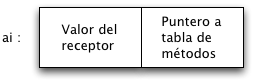
\includegraphics{oo/interface_value1.png} \end{center}
	
	En distintos momentos de la ejecución del programa posee distintos valores
	y tipo:
	
	\begin{verbatim} ai = &Punto { 3, 4 }  (== (*Punto) (0xff1234)):
	\end{verbatim}
	
	\begin{center} 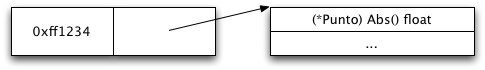
\includegraphics{oo/interface_value2.png} \end{center}
	
	\begin{verbatim} ai = MyFloat(-7.): \end{verbatim}
	
	\begin{center} 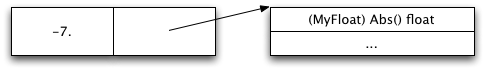
\includegraphics{oo/interface_value3.png} \end{center}
	
	\subsection{Hechos de los interfaces}
	
	Hay que tener en cuenta tres hecho sobre los interfaces en Go:
	
	\begin{enumerate} \item Los interfaces definen un conjunto de métodos. Son
	puros y completamente abstractos: No implementan nada, no tienen atributos.
	Go posee una clara separación entre interfaz e implementación.  \item Los
	valores de un interfaz son simplemente eso: valores. Contienen un valor
	concreto que implementa todos los métodos definidos en el interfaz.
	\textit{Dicho valor puede o puede no ser un puntero}.  \item Los tipos
	implementan interfaces simplemente teniendo sus métodos. No es necesario
	declarar explícitamente que lo hacen. Por ejemplo, como ya hemos visto,
	todos los tipos implementan \textit{EmptyInterface}.  \end{enumerate}
	
	\subsection{Ejemplo: io.Writer}
	
	El paquete \textit{io} concede una serie de métodos para el programador que
	pueden tratar la entrada y salida de datos. Para ver de forma más clara cómo
	son las interfaces, se ha elegido la interfaz \textit{io.Wirter} por ser
	bastante representativa y muy usada en Go.\\
	
	Si echamos un vistazo a la cabecera de la función \textit{Fprintf} del
	paquete \textit{fmt}, observamos que tiene la siguiente forma:
	
	\begin{verbatim} func Fprintf (w io.Writer, format string, a ...) (n int,
	error os.Error) \end{verbatim}
	
	Es decir, dicha función lo que recibe es una variable u objeto que sea de
	tipo io.Writer, no necesariamente un fichero donde escribir. El parámetro
	a de tipo ''...'' debería obviarse por ahora ya que se explicará más
	adelante. Como se puede observar, Fprintf devuelve una tupla con el número
	de caracteres escritos y el error en caso de que hubiera alguno.\\
	
	La interfaz io.Writer está definida de la siguiente manera:
	
	\begin{verbatim} type Writer interface { Write (p []byte) (n int, err
	os.Error) } \end{verbatim}
	
	Lo que quiere decir que todos los objetos que instancien dicha interfaz
	deberán tener un método Write que reciba un buffer de bytes y devuelva el
	número de caracteres escritos y un error en caso de que éste exista.\\
	
	Si echamos un vistazo al paquete \textit{bufio} que contiene métodos para
	realizar una entrada / salida con un buffer de datos, observamos que
	implementa un nuevo tipo de datos:

	\begin{verbatim} type Writer struct { ... } \end{verbatim}
	
	Implementando dicho tipo de datos (\textit{bufio.Writer}) el método
	\textit{Writer} canónico visto en el interfaz del mismo nombre.
	
	\begin{verbatim} func (b *Writer) Write (p []byte) (n int, err os.Error)
	\end{verbatim}
	
	Casi todos los paquetes de entrada / salida así como los que se encargan de
	la escritura en ficheros utilizan el interfaz Write. \\
	
	El paquete io tiene declarados 4 interfaces distintos, uno para cada uso
	distinto:
	
	\begin{itemize} \item Reader \item Writer \item ReadWriter \item
	ReadWriteCloser \end{itemize}
	
	\subsection{Comparación con C++}
	
	En C++ un tipo interfaz es como una clase abstracta pura, ya que se
	especifican los métodos pero no se implementa ninguno de ellos.\\
	
	En términos de Java, el tipo interfaz es mucho más parecido a una interfaz
	Java.\\
	
	En Go, hay una gran diferencia en un aspecto: Un tipo no necesita declarar
	las interfaces que implementa ni siquiera heredar de un tipo interfaz, sino
	que si tiene los métodos que definen el interfaz, entonces dicho tipo
	implementa el interfaz.
	
%	\subsection{Interfaces y atributos anónimos}	
	
%	\subsection{Ejemplo: Servicio HTTP}
	
	\subsection{Contenedores y la interfaz vacía}
	
	Los contenedores son estructuras de datos que permiten almacenar elementos
	de un determinado tipo o de cualquiera. Veamos cómo se realiza esto en una
	posible implementación de los vectores.  \clearpage \begin{verbatim} type
	Element interface {}
	   
	   //Vector es el propio contenedor type Vector struct { a []Element }
	   
	   // At() devuelve el i-ésimo elemento func (p *Vector) At(i int) Element
	   { return p.a[i] } \end{verbatim}
	
	Como se puede observar en el código anterior los vectores pueden contener
	elementos de cualquier tipo de datos ya que todos los tipos implementan la
	interfaz vacía (en este caso Element es una interfaz vacía). De hecho, cada
	elemento contenido en un vector podría ser de cualquier tipo.
	
	\subsection{Asertos de tipos}
	
	Una vez que se almacena un elemento en un \textit{Vector}, dicho elemento se
	almacena como un valor \textit{interfaz}. Es necesario por lo tanto
	``desempaquetarlo'' para tener el valor original, usando los asertos de
	tipos (o type assertions). Su sintaxis es:
	
	\begin{verbatim} valor_interfaz.(tipo_a_extraer) \end{verbatim}
	
	Veamos un ejemplo de cómo funcionarían los asertos:
	
	\begin{verbatim} var v vector.Vector
	   
	   v.Set (0, 1234.)  // Se guarda como un valor de interfaz i := v.At(0)
	   // Devuelve el valor como interface{}
	   
	   if i != 1234. {}            // Error en tiempo de compilación if
	   i.(float) != 1234. {}    // OK if i.(int) != 1234 {}       // Error en
	   tiempo de ejecución if i.(MyFloat) != 1234. {}  // Error: no es MyFloat
	   \end{verbatim}
	
	\subsection{Conversión de una interfaz a otra}
	
	Hasta ahora únicamente nos hemos limitado a mover valores normales dentro
	y fuera de valores interfaz, pero los valores de este tipo que contengan los
	métodos apropiados, también pueden ser convertidos a otros tipos de
	interfaces.\\
	
	De hecho, es lo mismo que desempaquetar el valor interfaz para extraer el
	valor concreto al que se hace referencia, para después volverlo a empaquetar
	para el nuevo tipo interfaz.\\
	
	La viabilidad de la conversión depende del valor referenciado, no del tipo
	original de la interfaz.\\
	
	Veamos un ejemplo de la conversión de intefaces, dadas las siguientes
	definiciones de variables y tipos:
	
	\begin{verbatim} var ai AbsInterface type SqrInterface interface { Sqr()
	float } var si SqrInterface pp := new(Point) // asumamos que *Point tiene
	Abs, Sqr var empty interface{} \end{verbatim}
	
	Todas estas operaciones serían correctas:
	
	\begin{verbatim} empty = pp  // Todo satisface empty ai
	= empty.(AbsInterface) // El valor referenciado // implementa Abs(). En
	cualquier otro // caso, produce un fallo en tiempo de ejecución.  si
	= ai.(SqrInterface)  // *Point tiene Sqr() // aunque AbsInterface no lo
	implemente empty = si // *Point implementa el conjunto vacío \end{verbatim}
	
	\subsection{Probando interfaces con asertos}
	
	En muchas ocasiones querremos saber con qué tipo de interfaz estamos
	tratando, es por ello que podemos gracias a los asertos preguntar qué tipo
	de interfaz tiene una determinada variable.\\
	
	Para ello se puede usar los asertos de tipo "coma ok":
	
	\begin{verbatim} elem := vector.At(0)
	   
	   if i, ok := elem.(int); ok { fmt.Printf ("int: \%d\n, i) } else if f, ok
	   := elem.(float); ok { fmt.Printf ("float: \%g\n", f) } else
	   { fmt.Print("tipo desconocido\n") } \end{verbatim} \clearpage También
	   podemos comprobar los interfaces con un switch de tipos:
	
	\begin{verbatim} switch v := elem.(type) {  // Literal "type" case int:
	fmt.Printf ("int: \%d\n", v) case float: fmt.Printf ("float: \%g\n", v)
	default: fmt.Print("tipo desconocido\n") \end{verbatim}
	
	Y yendo un paso más allá, podemos preguntar si un valor de tipo interfaz
	implementa un método. De esta forma, por ejemplo, es como \textit{Print}
	decide si el tipo puede imprimirse así mismo o si debe usar una
	representación genérica del mismo.
	
	\begin{verbatim} type Stringer interface { String() string }
	   
	   if sv, ok := v.(Stringer); ok { fmt.Printf("implementa String(): \%s\n",
	   sv.String()) } \end{verbatim}
	
	\subsection{El paquete reflect}
	
	En Go existe un paquete \textit{reflect} que utiliza la misma base de
	determinar los tipos de los parámetros en las llamadas a las funciones
	usando los asertos. Así es posible usar un nuevo argumento ''...'' que
	permite pasar argumentos indefinidos a una función. Veamos un ejemplo con
	\textit{Printf}:
	
	\begin{verbatim} func Printf (format string, args ...) (n int, err os.Error)
	\end{verbatim}
	
	El argumento ''...'' usado dentro de Printf (o en cualquier otro sitio)
	tiene el tipo \textit{interface\{\}}, y \textit{Printf} usa el paquete
	\textit{reflect} para desempaquetar y descubrir la lista de argumentos.\\
	
	Como resultado, tenemos que toda la familia de funciones \textit{Print}
	saben los tipos de todos sus argumentos. Como conocen si el argumento es
	unsigned o long, no hay necesidad de \textit{\%u} o \textit{\%ld},
	simplemente \textit{\%d}, simplificando mucho la lista de modificadores.
	
